% !TEX TS-program = pdflatex
% !TEX root = ../ArsClassica.tex

%************************************************
\chapter{Development Environment}
\label{chp:1-Environment}
%************************************************
To allow replicability of our experiments, we have added some information about the system and the environment that we used for the following research. 
We used the following development environment:
\begin{itemize}
\item \textsc{CPLEX} :  version 0.1-2018
\item \textsc{Linux Ubuntu} : version 18.04 LTS (Operative System)
\item \textsc{C}  	(language)
\item \textsc{Sublime text} (IDE / text editor)
\item \textsc{Github} (web-based version control using Git)
\item \textsc{Gnuplot} (library plot)
\end{itemize}

\section{Real World Info}
As in \cite{wfcp} research, we used a library of real-life instances that are publicly available for benchmarking.
For benchmark purposes, we collected the data of five real wind farms in operation in United Kingdom (wf02, wf03, wf05) and Denmark (wf01, wf04). Different types of cable with different costs, capacities and electrical resistances are available on the market; we considered 5 sets of real cables, named cb01, cb02, cb03, cb04, and cb05. The turbines in each wind park are of the same type, so we can express the cable capacities as the maximum number of turbines that it can support. Finally, we list the maximum number of connections to the substation, or to be specific, the input parameter C. The table 1 contains all the information.
\begin{table}[!htbp]\label{tab:realWorld}
\center
\begin{tabular}{llllll}
\hline
name & site         & turbine type  & no. of turbines & C  & allowed cables      \\ \hline
wf01 & Horn Rev 1   & Vestas 80-2MW & 80              & 10 & cb01-cb02-cb05      \\
wf02 & Kentis Flats & Vestas 90-3MW & 30              & $\infty$   & cb01-cb02-cb04-cb05 \\
wf03 & Ormonde      & Senvion 5MW   & 30              & 4  & cb03-cb04           \\
wf04 & DanTysk      & Simens 3.6MV  & 80              & 10 & cb01                \\
wf05 & Thanet       & Vestas 90-3MW & 100             & 10 & cb04-cb05           \\ \hline
\end{tabular}
\caption{Basic information on the real-world wind farms that were used for testing.}
\end{table}

\section{Instance TEST BED}
The test that we were able to use are the combinations between the 5 instances of wind farms and the 5 sets of real cables. For simplicity reasons and in order to eliminate mistakes, we adopted the same a numeration as the \cite{wfcp} article. This solution allows us to easily compare our results with the results in that research. 
Table 2 reports the resulting numbers of the different instances. For example we renamed the 01 wind farm as \textit{data\_01.turb} and the corresponding cables as \textit{data\_01.cbl}. Images \ref{img:ex1} and \ref{img:ex2} shows two instances from TEST BED.

\begin{table}[!htbp]\label{tab:testBed}
\center
\begin{tabular}{lcl}
\hline
number & \multicolumn{1}{l}{wind farm} & cable set         \\ \hline
01     & \multirow{6}{*}{wf01}         & wf01\_cb01\_capex \\
02     &                               & wf01\_cb01        \\
03     &                               & wf01\_cb02\_capex \\
04     &                               & wf01\_cb02        \\
05     &                               & wf01\_cb05\_capex \\
06     &                               & wf01\_cb05        \\ \hline
07     & \multirow{8}{*}{wf02}         & wf02\_cb01\_capex \\
08     &                               & wf02\_cb01        \\
09     &                               & wf02\_cb02\_capex \\
10     &                               & wf02\_cb02        \\
12     &                               & wf02\_cb04\_capex \\
13     &                               & wf02\_cb04        \\
14     &                               & wf02\_cb05\_capex \\
15     &                               & wf02\_cb05        \\ \hline
16     & \multirow{4}{*}{wf03}         & wf03\_cb03\_capex \\
17     &                               & wf03\_cb03        \\
18     &                               & wf03\_cb04\_capex \\
19     &                               & wf03\_cb04        \\ \hline
20     & \multirow{2}{*}{wf04}         & wf04\_cb01\_capex \\
21     &                               & wf04\_cb01        \\ \hline
26     & \multirow{4}{*}{wf05}         & wf05\_cb04\_capex \\
27     &                               & wf05\_cb04        \\
28     &                               & wf05\_cb05\_capex \\
29     &                               & wf05\_cb05        \\ \hline
\end{tabular}
\caption {Test Bed instance numbers.}
\end{table}

\begin{minipage}{7cm} 
	\centering
	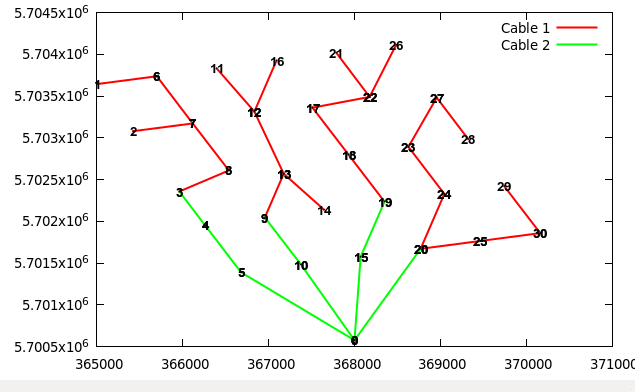
\includegraphics[scale=0.3]{Graphics/data07.png} \\
	\captionof{figure}{Example of problem: data07}
	\label{img:ex1}
	\end{minipage}
	\begin{minipage}{7cm} 
	\centering
	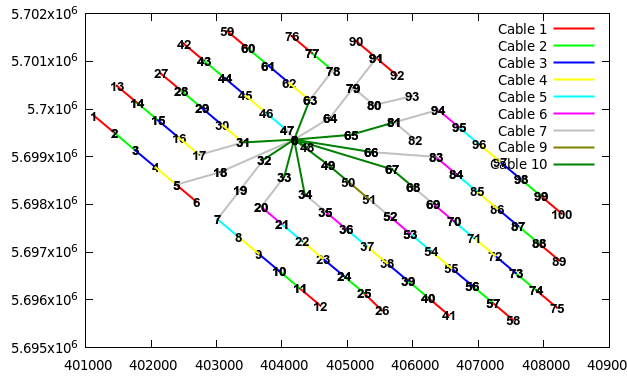
\includegraphics[scale=0.3]{Graphics/data29.png} \\
	\captionof{figure}{Example of problem: data29}
	\label{img:ex2}
	\end{minipage}

\newpage